\documentclass{beamer}
\usepackage{dsfont}

\mode<presentation> {

%\usetheme{default}
%\usetheme{AnnArbor}
%\usetheme{Antibes}
%\usetheme{Bergen}
%\usetheme{Berkeley}
%\usetheme{Berlin}
%\usetheme{Boadilla}
%\usetheme{CambridgeUS}
%\usetheme{Copenhagen}
%\usetheme{Darmstadt}
%\usetheme{Dresden}
%\usetheme{Frankfurt}
%\usetheme{Goettingen}
%\usetheme{Hannover}
%\usetheme{Ilmenau}
%\usetheme{JuanLesPins}
%\usetheme{Luebeck}
\usetheme{Madrid}
%\usetheme{Malmoe}
%\usetheme{Marburg}
%\usetheme{Montpellier}
%\usetheme{PaloAlto}
%\usetheme{Pittsburgh}
%\usetheme{Rochester}
%\usetheme{Singapore}
%\usetheme{Szeged}
%\usetheme{Warsaw}

%\usecolortheme{albatross}
%\usecolortheme{beaver}
%\usecolortheme{beetle}
%\usecolortheme{crane}
%\usecolortheme{dolphin}
%\usecolortheme{dove}
%\usecolortheme{fly}
%\usecolortheme{lily}
%\usecolortheme{orchid}
%\usecolortheme{rose}
%\usecolortheme{seagull}
%\usecolortheme{seahorse}
%\usecolortheme{whale}
%\usecolortheme{wolverine}

%\setbeamertemplate{footline} % To remove the footer line in all slides uncomment this line
%\setbeamertemplate{footline}[page number] % To replace the footer line in all slides with a simple slide count uncomment this line

%\setbeamertemplate{navigation symbols}{} % To remove the navigation symbols from the bottom of all slides uncomment this line
}

\usepackage{graphicx} % Allows including images
\usepackage{booktabs} % Allows the use of \toprule, \midrule and \bottomrule in tables
\usepackage[backend=biber, bibencoding=utf8]{biblatex}
\usepackage[ruled, vlined]{algorithm2e}
\setbeamercovered{transparent}
\bibliography{references.bib}

%----------------------------------------------------------------------------------------
%	TITLE PAGE
%----------------------------------------------------------------------------------------

\title{Random Forest for Classification Problems} % The short title appears at the bottom of every slide, the full title is only on the title page

\author{Raphael, Arkadiusz and  Burak} % Your name
\institute[Uni Bonn] % Your institution as it will appear on the bottom of every slide, may be shorthand to save space
{
Uni Bonn \\ % Your institution for the title page
\medskip
}
\date{\today} % Date, can be changed to a custom date

\begin{document}

\begin{frame}
    \titlepage % Print the title page as the first slide
\end{frame}

\begin{frame}
\frametitle{Overview} % Table of contents slide, comment this block out to remove it
\tableofcontents % Throughout your presentation, if you choose to use \section{} and \subsection{} commands, these will automatically be printed on this slide as an overview of your presentation
\end{frame}

%----------------------------------------------------------------------------------------
%	PRESENTATION SLIDES
%----------------------------------------------------------------------------------------

%%------------------------------------------------
\section{Intro} % Sections can be created in order to organize your presentation into discrete blocks, all sections and subsections are automatically printed in the table of contents as an overview of the talk
%------------------------------------------------

% \subsection{Subsection Example} % A subsection can be created just before a set of slides with a common theme to further break down your presentation into chunks

\begin{frame}
\frametitle{Intro}
Sed iaculis dapibus gravida. Morbi sed tortor erat, nec interdum arcu. Sed id lorem lectus. Quisque viverra augue id sem ornare non aliquam nibh tristique. Aenean in ligula nisl. Nulla sed tellus ipsum. Donec vestibulum ligula non lorem vulputate fermentum accumsan neque mollis.\\~\\

Sed diam enim, sagittis nec condimentum sit amet, ullamcorper sit amet libero. Aliquam vel dui orci, a porta odio. Nullam id suscipit ipsum. Aenean lobortis commodo sem, ut commodo leo gravida vitae. Pellentesque vehicula ante iaculis arcu pretium rutrum eget sit amet purus. Integer ornare nulla quis neque ultrices lobortis. Vestibulum ultrices tincidunt libero, quis commodo erat ullamcorper id.
\end{frame}

%------------------------------------------------

\section{Decision Tree}

\begin{frame}
	\frametitle{Decision Tree}
	\begin{block}{Block 1}
	Lorem ipsum dolor sit amet, consectetur adipiscing elit. Integer lectus nisl, ultricies in feugiat rutrum, porttitor sit amet augue. Aliquam ut tortor mauris. Sed volutpat ante purus, quis accumsan dolor.
	\end{block}
	
	\begin{block}{Block 2}
	Pellentesque sed tellus purus. Class aptent taciti sociosqu ad litora torquent per conubia nostra, per inceptos himenaeos. Vestibulum quis magna at risus dictum tempor eu vitae velit.
	\end{block}
	
	\begin{block}{Block 3}
	Suspendisse tincidunt sagittis gravida. Curabitur condimentum, enim sed venenatis rutrum, ipsum neque consectetur orci, sed blandit justo nisi ac lacus.
	\end{block}
\end{frame}


\section{Bias Variance}

\begin{frame}
    \frametitle{Bias Variance}
    \begin{columns}[c] % The "c" option specifies centered vertical alignment while the "t" option is used for top vertical alignment
    
    \column{.45\textwidth} % Left column and width
    \textbf{Heading}
    \begin{enumerate}
    \item Statement
    \item Explanation
    \item Example
    \end{enumerate}
    
    \column{.5\textwidth} % Right column and width
    Lorem ipsum dolor sit amet, consectetur adipiscing elit. Integer lectus nisl, ultricies in feugiat rutrum, porttitor sit amet augue. Aliquam ut tortor mauris. Sed volutpat ante purus, quis accumsan dolor.
    
    \end{columns}
\end{frame}

\subsection{Bagging}

\begin{frame}
    \frametitle{Bagging}

	Bagging is:
    \begin{enumerate}
    \item created for methods with high variance
    \item reduces variance and gives better predictions
    \item improvement of bagging: Random Forest
    \end{enumerate}
    

\end{frame}

\begin{frame}
    \frametitle{Bagging}

	\begin{center}		
		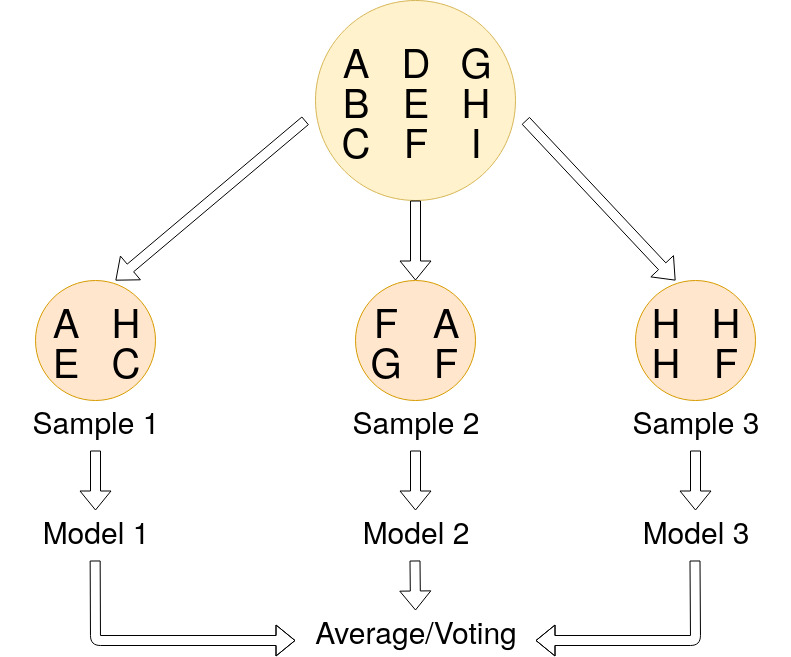
\includegraphics[height=0.7\textheight]{images/bagging_1.jpg}
	\end{center}

\end{frame}

%------------------------------------------------
\section{Random Forest}
%------------------------------------------------

\begin{frame}
\frametitle{Random Forest}
%\begin{table}
%\begin{tabular}{l l l}
%\toprule
%\textbf{Treatments} & \textbf{Response 1} & \textbf{Response 2}\\
%\midrule
%Treatment 1 & 0.0003262 & 0.562 \\
%Treatment 2 & 0.0015681 & 0.910 \\
%Treatment 3 & 0.0009271 & 0.296 \\
%\bottomrule
%\end{tabular}
%\caption{Table caption}
%\end{table}

An ensemble of randomly trained decision trees, so in other words 
random forest was defined by L. Breiman:
\vspace{1ex}

\begin{theorem}
	A random forest is a classifier consisting of a collection of tree-structured classifiers ${\hat{T}_{\theta_{b}}(\textbf{x})}, b = 1,...,B$ where the $\theta_{b}$ are independent identically
	distributed random vectors and each tree casts a unit vote for the most popular class at input $\textbf{x}$ .
\end{theorem}
\vspace{4ex}

Random Forest is an extension and improvement over bagging:
\begin{enumerate}
\item Like in bagging, multiple decision trees are built
\item Improvement: an injection of randomness is made
\end{enumerate}

\end{frame}

%------------------------------------------------

\begin{frame}
\frametitle{Random Forest: randomness in the model}

Two key concepts that makes decision forest "random" are:
\begin{enumerate}
	\item Random sampling of training data points when building trees
	\item Random subsets of features considered when splitting nodes. Recommended number of variables:
	\begin{enumerate}[a]
	    \item For classification:  $\lfloor{\sqrt{n}} \rfloor$
	    \item For regression: $\lfloor \frac{n}{3} \rfloor$
	\end{enumerate}
\end{enumerate}


\end{frame}

\begin{frame}
\frametitle{Random Forest: algorithm}

\begin{algorithm}[H]
\SetAlgoLined
\begin{enumerate}
	\item For $b$ = 1 to $B$:
	\begin{enumerate}[a]
	    \item Draw a bootstrap sample $\theta_{b}$ of size N from the training data.
	    \item Grow the Random Forest tree ${{T}_{\theta_{b}}}$ to the bootstrapped data, by recursively repeating the following steps for each terminal node of the tree, until the minimum node size $n_{min}$ is reached:
	    \begin{enumerate}[i]
	       \item Select $m$ variables at random from the $n$ variables
	       \item Pick the best variable/split-point among the $m$
	       \item  Split the node into two daughter nodes
	    \end{enumerate}
	\end{enumerate}
	\item  Output the ensemble of trees $\{{T}_{\theta_{b}}\}_{1}^{B}$
\end{enumerate}
 \caption{Random Forest for Regression or Classification}
\end{algorithm}

\end{frame}

















\section{Mathematical Concept}

\begin{frame}
    \frametitle{Mathematical Explanation}
    Let $D = \{(x_{1},y_{1}), (x_{2}, y_{2}), ... , (x_{N}, y_{N})\}$ 
    and $T_{D,\theta}$ is fully grown decision tree trained on set $D$ with using parameters $\theta$.
    Random Forest estimate of an observation $x^*$ is
    \begin{block}{Majority Voting}
        \begin{equation}
            \boldsymbol{RF}_{D, \theta_{1}, \theta_{2}, ..., \theta_{B}} (x^*) =
            \underset{c \in Y}{argmax} \sum_{b = 1}^{B}{1(\hat{T}_{b}(x^*) = c)}
        \end{equation}
    \end{block}
    \begin{block}{Soft Voting}
        \begin{equation}
            \boldsymbol{RF}_{D, \theta_{1}, \theta_{2}, ..., \theta_{B}} (x^*) =
            \underset{c \in Y}{argmax} \dfrac{1}{B}\sum_{b = 1}^{B}{\hat{p}_{D, \theta_{b}} (Y = c | X = x^*)}
        \end{equation}
    \end{block}
    where $\hat{p}_{D, \theta_{b}} (Y = c | X = x^*)$ is the probability estimates of a tree.
\end{frame}
\begin{frame}
    \frametitle{Majority Voting}
    \begin{figure}
        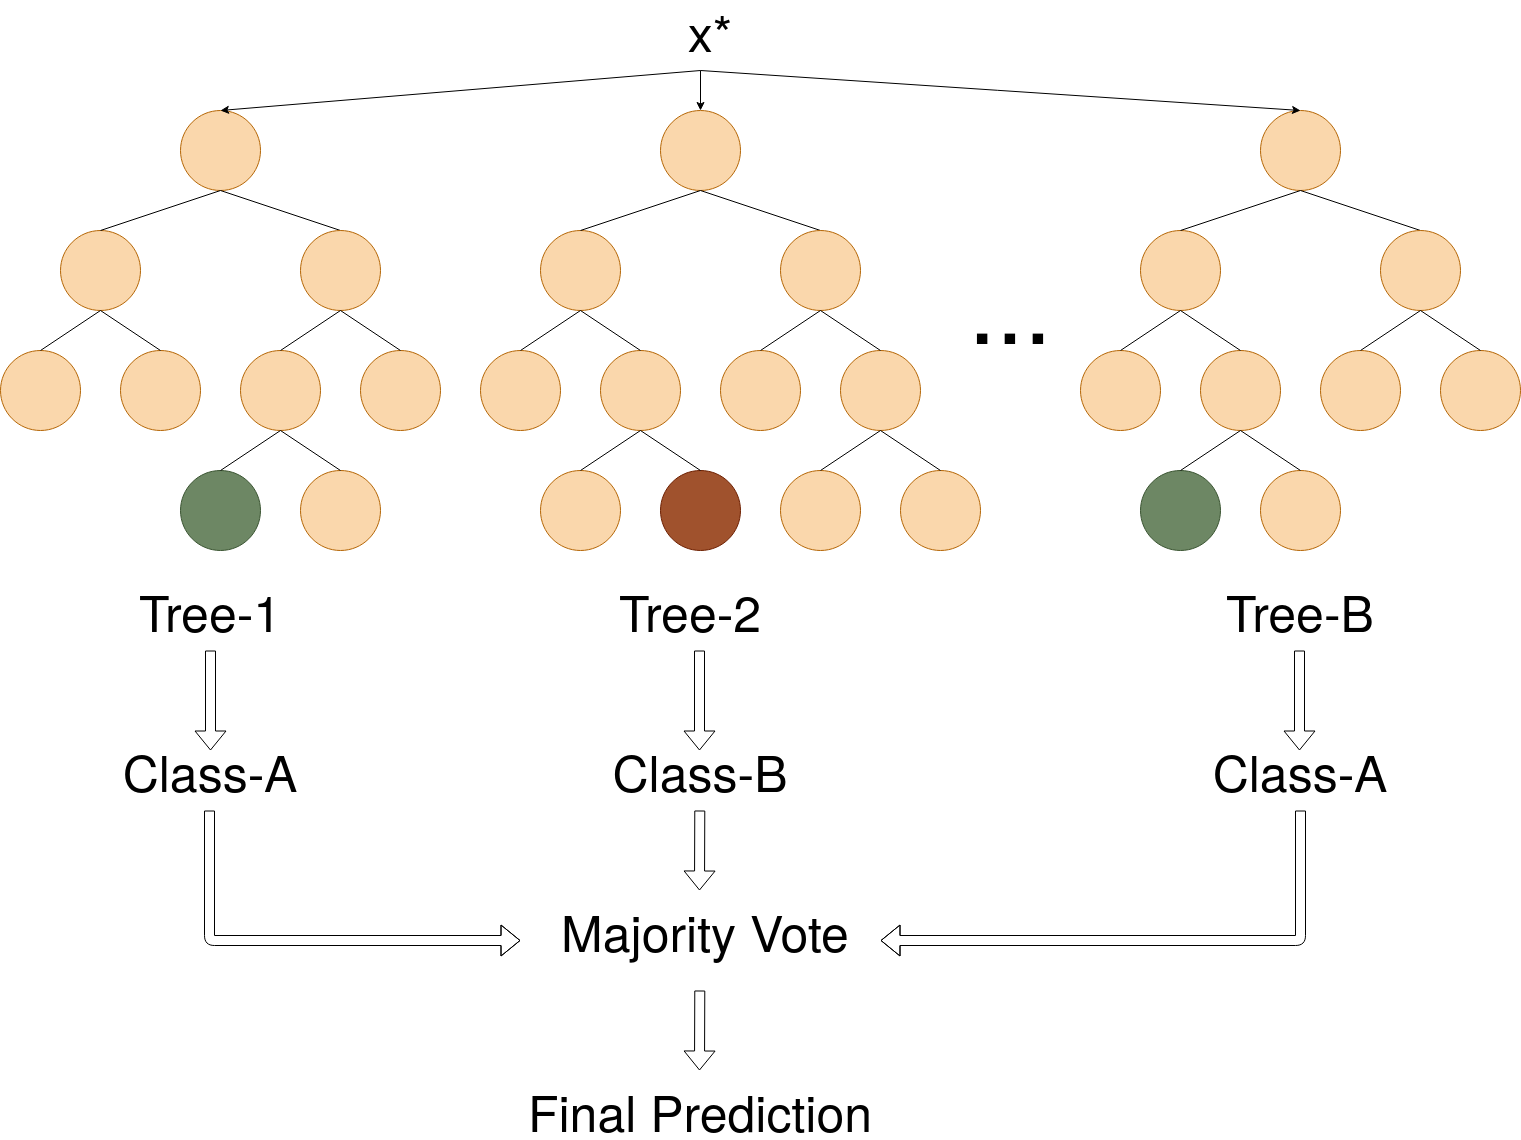
\includegraphics[height=0.7\textheight]{images/majority.png}
        \caption{Majority Voting Illustration}
    \end{figure}
\end{frame}
\begin{frame}
    \frametitle{Soft Voting}
    \begin{figure}
    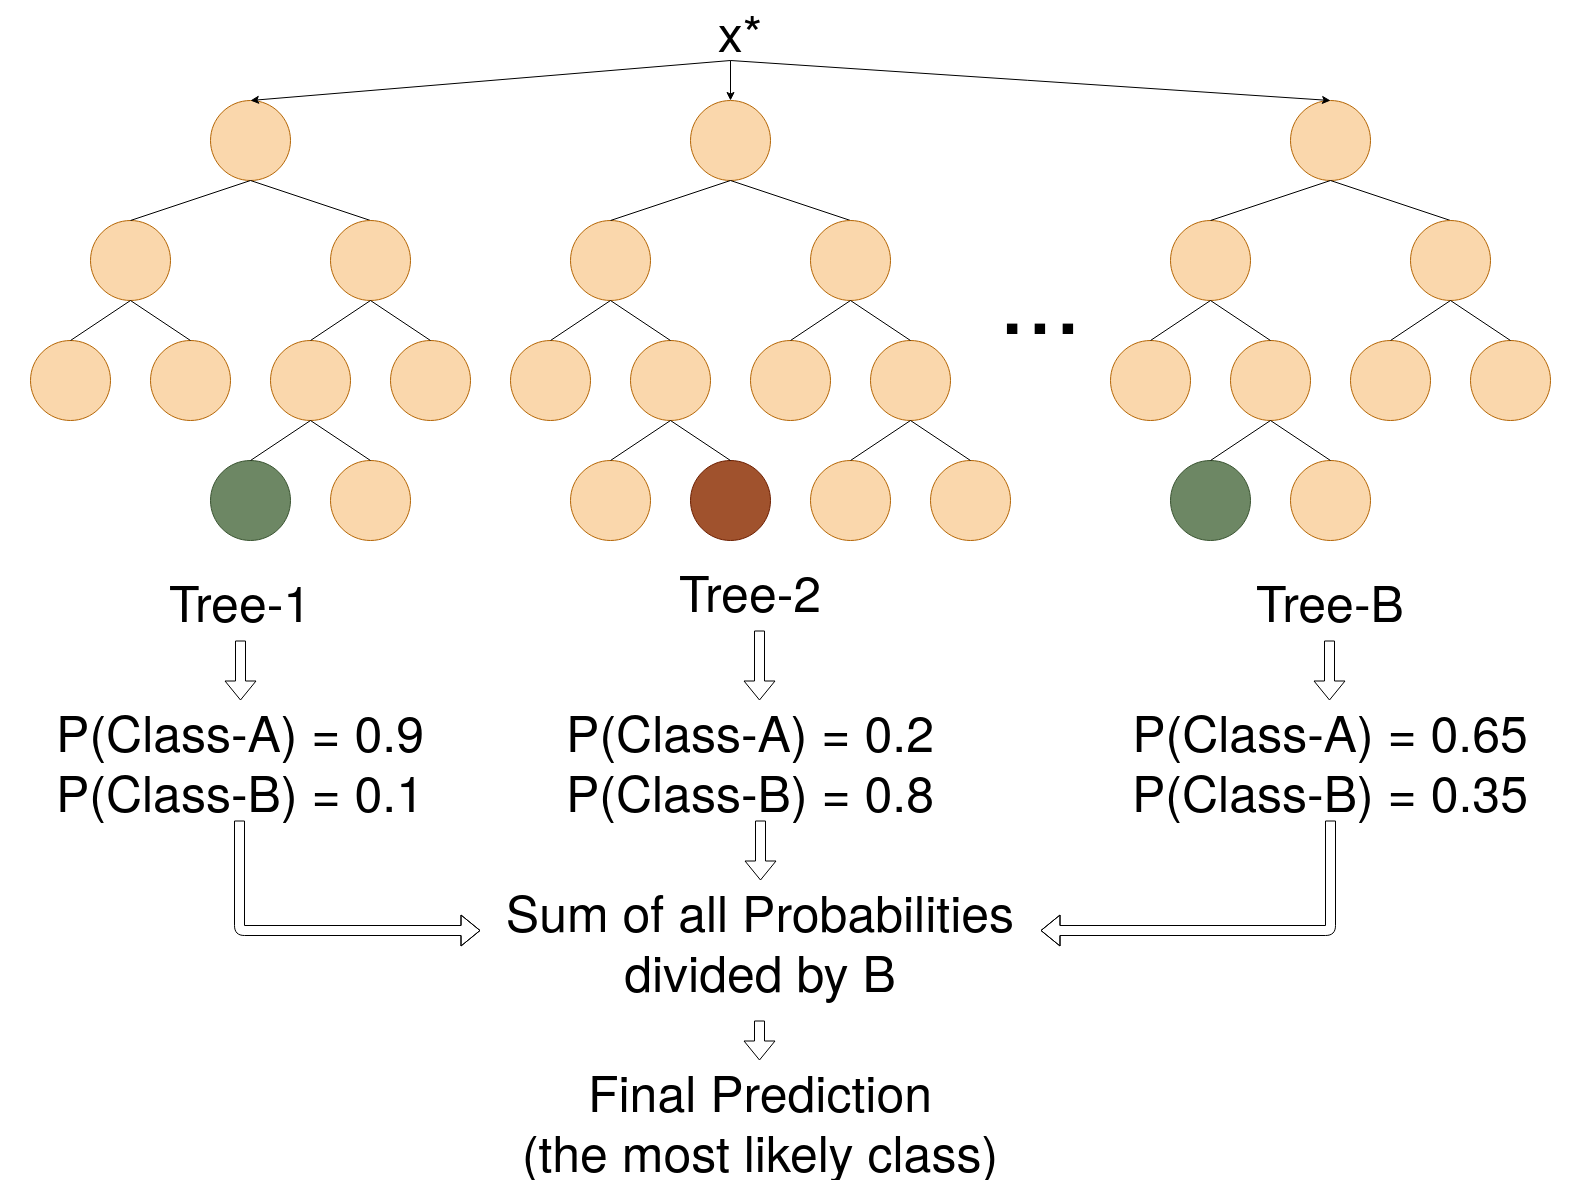
\includegraphics[height=0.7\textheight]{images/soft.png}
    \caption{Soft Voting Illustration}
    \end{figure}
\end{frame}
\begin{frame}
    \frametitle{Bayes Model}
    Theoretically, there exists a model that minimizes the generalization error and can be derived analitically independent of the model \cite{louppe2014understanding}.
    Conditioning the expected generalization error on X gives:
    \begin{equation}
        \mathbb{E}_{X,Y} \{L(Y, \phi_{\beta}(X))\} = \mathbb{E}_{X}\{\mathbb{E}_{Y|X}\{L(Y, \phi_{\beta}(X)) \} \}
    \end{equation}
    Point-wise minimization of inner term yields:
    \begin{equation}
        \phi_{\beta} = \underset{c \in Y}{argmin} \; \mathbb{E}_{Y|X=x}\{L(Y,c)\}
    \end{equation}
    $\phi_{\beta}$ is Bayes Model and as mentioned $\boldsymbol{Err}(\phi_{\beta})$ is the irreducible error.
\end{frame}
\begin{frame}
    \frametitle{The Expected Generalization Error}
        The expected generalization error of $T_{D,\theta}$ is
        \begin{equation}\label{eq:exp_gen_error}
            \boldsymbol{Err}(T_{D,\theta}) = \mathbb{E}_{X,Y}\{L(Y, T_{D,\theta}(X)) \}
        \end{equation}
        with the decomposition as
        \begin{equation}
        \boldsymbol{Err}(T_{D,\theta}) = noise(x) + bias^2(x) + var(x)
    \end{equation}
    \qquad \quad where
    \begin{align}
        & noise(x) = \boldsymbol{Err}(\phi_{\beta}) \notag \\
        & bias^2(x) = (\phi_{\beta}(x) - \mathbb{E}_{D}\{T_{D,\theta}(x)\})^2 \notag \\
        & var(x) = \mathbb{E}_{D}\{(\mathbb{E}_{D}(T_{D,\theta}(x)) - T_{D,\theta}(x))^2\} \notag
    \end{align}
\end{frame}
%\begin{frame}
%    \frametitle{Loss Functions}
%\begin{block}{Regression}
%            Squared Loss Function
%            \begin{align}
%                L(Y, T_{D, \theta}(x)) = (Y - T_{D, \theta}(x))^2\\
%                \boldsymbol{Err}(T_{D,\theta}) = \mathbb{E}_{X,Y}\{ (Y - T_{D, \theta}(x))^2 \}
%            \end{align}
%        \end{block}
%\begin{block}{Classification}    
%            Zero-One Loss Function
%            \begin{align}
%                L(Y, T_{D,\theta}(X)) = 1 (Y \neq T_{D, \theta}(X))
%            \end{align}                
%            \begin{align}
%                \boldsymbol{Err'}(T_{D,\theta}) & = \mathbb{E}_{X,Y}\{ 1(Y \neq T_{D, \theta}(X)) \}\notag \\
%                & = P(Y \neq T_{D, \theta}(X))
%            \end{align}
%        \end{block}
%\end{frame}
%\begin{frame}
%    \frametitle{Bayes Model cont.}
%    \begin{block}{Regression}
%        \begin{align}
%            \phi_{\beta} & = \underset{c \,\in\, Y}{argmin} \; \mathbb{E}_{Y|X=x}\{(Y-c)^2 \} \notag\\
%            \phi_{\beta} & = \mathbb{E}_{Y|X=x}\{Y\}\\
%            \boldsymbol{Err}(\phi_{\beta}) & = \mathbb{E}_{Y|X=x}\{(Y-\phi_{\beta}(x))^2 \}
%        \end{align}
%    \end{block}
%    \begin{block}{Classification}
%        \begin{align}
%            \phi_{\beta}' & = \underset{c \,\in\, Y}{argmin} \; \mathbb{E}_{Y|X=x}\{L(Y,c) \} \notag\\
%            \phi_{\beta}' & = \underset{c \,\in\, Y}{argmax} \; P(Y = c \,| X = x)\\
%            \boldsymbol{Err}(\phi_{\beta}') & = P(Y \neq \phi_{\beta}'(x) )
%        \end{align}
%    \end{block}
%\end{frame}

\begin{frame}
    \frametitle{Random Forest}
    Random Forest Estimator for regression shares the same idea with soft-voting classification;
    \begin{equation}
        \boldsymbol{RF}_{D, \theta_{1},\theta_{2},..., \theta_{B}}(x) = \dfrac{1}{B}\sum_{b = 1}^{B}T_{D,\theta_{b}}(x)
    \end{equation}
    Taking expectation gives;
    \begin{align}
        \mathbb{E}_{D, \theta_{1}, \theta_{2},..., \theta_{B}}\{\boldsymbol{RF}_{D, \theta_{1},\theta_{2},..., \theta_{B}}(x) \} 
        & = \mathbb{E}_{D, \theta_{1}, \theta_{2},..., \theta_{B}}\{\dfrac{1}{B}\sum_{b = 1}^{B}T_{D,\theta_{b}}(x)\} \notag \\
        & = \dfrac{1}{B}\sum_{b=1}^{B}\mathbb{E}_{D,\theta_{b}}\{T_{D, \theta_{b}}(x)\}\notag \\
        & = \mu_{D,\theta}(x)
    \end{align}
    where $\mu_{D,\theta}(x)$ is the average prediction of all ensembled trees.
\end{frame}
\begin{frame}
    \frametitle{$Bias^2$ of Random Forest}
    $Bias^2$ of a tree in regression setting
    \begin{equation}
        [bias(T_{D,\theta})(x)]^2 = (\phi_{\beta}(x) - \mathbb{E}_{D}\{T_{D,\theta}(x)\})^2
    \end{equation}
    When we extend our findings to Random Forest;
    \begin{equation}
        [bias(\boldsymbol{RF}_{D,\theta})(x)]^2 = (\phi_{\beta}(x) - \mu_{D,\theta}(x))^2
    \end{equation}
\end{frame}
\begin{frame}
    \frametitle{Correlation Coefficient}
    For any two trees $T_{D,\theta'}$ and $T_{D,\theta''}$ trained with the same data $D$
    and different growing parameters $\theta'$ and $\theta''$, we can define the correlation coefficient as follows
    \begin{align}
        \rho(x) & 
        = \dfrac{\mathbb{E}_{D,\theta',\theta''}\{T_{D,\theta'}(x) T_{D,\theta''}(x)\} 
        - \mu_{D,\theta}^2(x)}{\sigma_{D,\theta}^2(x)}
    \end{align}
    $\rho(x)$ is close to 1 $\implies$ highly correlated trees and randomization has no significant effect. \\
    $\rho(x)$ is close to 0 $\implies$ non-correlated and perfectly random prediction of two trees
\end{frame}
\begin{frame}
    \frametitle{Variance of Random Forest}
    \begin{align}
        \mathbb{V}_{D, \theta_{1}, \theta_{2},..., \theta_{B}}\{\boldsymbol{RF}_{D, \theta_{1},\theta_{2},..., \theta_{B}}(x) \}  = \rho(x)\sigma^2_{D,\theta}(x) + \dfrac{1-\rho(x)}{B}\sigma^2_{D,\theta}(x)
    \end{align}
    \bigbreak
    \quad As $B \rightarrow \infty$, $\mathbb{V}\{\boldsymbol{RF}_{D, \theta_{1},\theta_{2},..., \theta_{B}}(x) \}$ converges to $\rho(x)\sigma^2_{D,\theta}(x)$.\\
    \bigbreak
    \quad Due to randomization $\rho(x) < 1 \implies \mathbb{V}\{\boldsymbol{RF}_{D, \theta_{1},\theta_{2},..., \theta_{B}}(x) \}< \sigma^2_{D,\theta}(x)$.
\end{frame}



\section{Simulation Study}
\frame{\sectionpage}
\frametitle{Simulation Study}
\begin{frame}
    \frametitle{Simulation Study}
    \framesubtitle{Linear DGP}
    The linear DGP generates the data tuples \( (y, x_{1}, x_{2}, x_{3}) \) as follows:

    \begin{equation*}\label{eq:linear_dgp}
        y = \beta_{0} + \beta_{1} x_{1} + \beta_{2} x_{2} + \beta_{3} x_{3} + \epsilon,
    \end{equation*}
    
    whereas
    \begin{itemize}
        \item $ \irow{\beta_{0} & \beta_{1} & \beta_{2} & \beta_{3}} = \irow{0.3 & 5 & 10 & 15}$
        \item $x_{1}, x_{2}, x_{3} \sim \mathcal{N}(0,\,3)$
        \item $\epsilon \sim \mathcal{N}(0,\,1)$
    \end{itemize}
\end{frame}

\begin{frame}
    \frametitle{Simulation Study}
    \framesubtitle{Linear DGP Results}
	\begin{center}		
		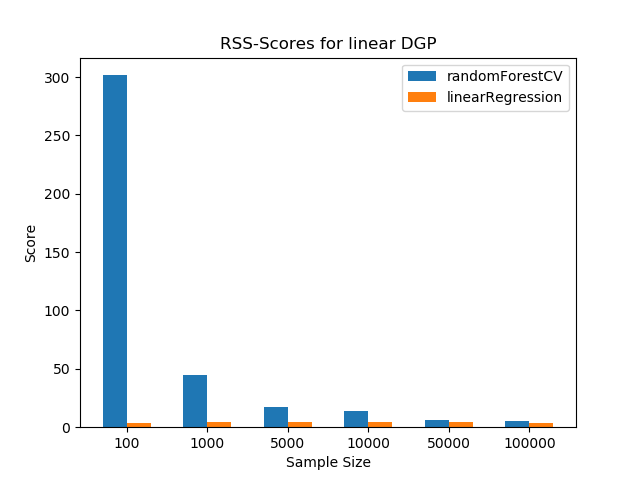
\includegraphics[height=0.7\textheight]{images/forest_vs_ols_linearDGP.png}
	\end{center}
\end{frame}


\begin{frame}
    \frametitle{Simulation Study}
    \framesubtitle{Non-Linear DGP}
    The non-linear DGP generates the data tuples \( (y, x_{1}, x_{2}) \) as follows:

    \begin{equation*}\label{eq:non_linear_dgp}
        y = \beta_{0} + \beta_{1} \mathds{1}(x_{1} \geq 0, x_{2} \geq 0) + \beta_{2} \mathds{1}(x_{1} \geq 0, x_{2} < 0) + \beta_{3} \mathds{1}(x_{1} < 0) + \epsilon,
    \end{equation*}
    
    whereas
    \begin{itemize}
        \item $ \irow{\beta_{0} & \beta_{1} & \beta_{2} & \beta_{3}} = \irow{0.3 & 5 & 10 & 15}$
        \item $x_{1}, x_{2} \sim \mathcal{N}(0,\,3)$
        \item $\epsilon \sim \mathcal{N}(0,\,1)$
    \end{itemize}
    are the same as in the previous DGP.
\end{frame}

\begin{frame}
    \frametitle{Simulation Study}
    \framesubtitle{Non-Linear DGP Results}
	\begin{center}		
		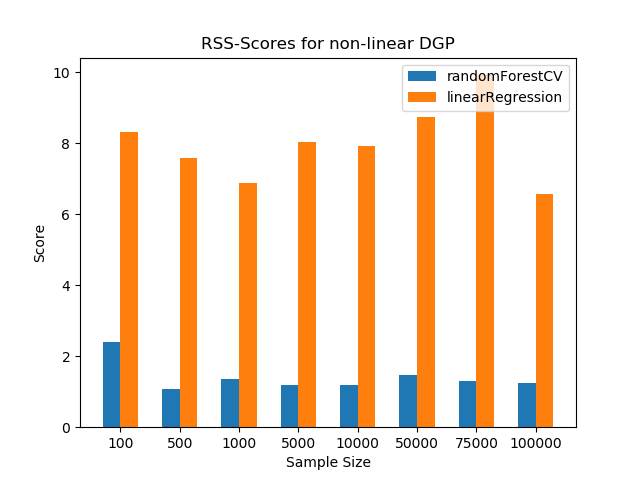
\includegraphics[height=0.7\textheight]{images/forest_vs_ols_nonlinearDGP.png}
	\end{center}
\end{frame}

\section{Real Data}

\begin{frame}[fragile] % Need to use the fragile option when verbatim is used in the slide
    \frametitle{Real Data}
    \textbf{Data}: Titanic data
\vspace{1ex}
    \newline \textbf{Method used}: 
\vspace{1ex}
    \begin{enumerate}
        \item Random Forest
        \item Adaptive Boosting 
        \item Gradient Boosting
    \end{enumerate}
\vspace{1ex}
    \textbf{Goal}: Predict which passengers survived the Titanic shipwreck given characteristics of passengers
\end{frame}
    
%------------------------------------------------

\begin{frame}[fragile] % Need to use the fragile option when verbatim is used in the slide
    \frametitle{Real Data}
    \framesubtitle{Results}
 
\begin{columns}[c] % The "c" option specifies centered vertical alignment while the "t" option is used for top vertical alignment
    \column{.33\textwidth} % Left column and width
    Random Forest
\vspace{1ex}
    \newline Accuracy: ~84.32\%
\vspace{2ex}

    
\begin{table}
\centering
\begin{tabular}{lll}
  & $D_{pred}$ & $S_{pred}$    \\
$D_{real}$ & 88\%   &  12\%\\
$S_{real}$ & 21\%& 79\%   \\

\end{tabular}
\end{table}


    \column{.33\textwidth} % Central column and width
    Adaptive Boosting
\vspace{1ex}
    \newline Accuracy: ~82.8\%
\vspace{2ex}

\begin{table}
\centering
\begin{tabular}{lll}
  & $D_{pred}$ & $S_{pred}$    \\
$D_{real}$ & 86\%   &   14\%\\
$S_{real}$ &  21\% & 79\%   \\

\end{tabular}
\end{table}

	
    \column{.33\textwidth} % Right column and width
    Gradient Boosting
\vspace{1ex}
    \newline Accuracy: ~82.8\%
\vspace{2ex}

\begin{table}
\centering
\begin{tabular}{lll}
  & $D_{pred}$ & $S_{pred}$    \\
$D_{real}$ & 85\%   &  15\%\\
$S_{real}$ &  20\% &    80\%\\

\end{tabular}
\end{table}


    \end{columns}
\end{frame}

\section{Conclusion}

\begin{frame}
    \frametitle{Conclusion}
    \Huge{\centerline{The End}}
\end{frame}
    
%---------------------------------------------------------------------------------------

\section{References}

\begin{frame}
    \frametitle{References}
    \footnotesize{

    \printbibliography
    }
\end{frame}

\end{document} 